
\newpage
\section{Injection SQL}
L'injection SQL est une des attaques les plus dangereuses.  

\subsection{Description}

\subsection{Exploitation}

\subsection{Contre-mesure}


\section{Injection SQL aveugle}
Blind SQL Injection 
\subsection{Description}

\subsection{Exploitation}

\subsection{Contre-mesure}


\section{Attaques XSS }

\subsection{Description}

\subsection{Exploitation}

\subsection{Contre-mesure}


\section{Attaques XSS enregistrées }

\subsection{Description}

\subsection{Exploitation}

\subsection{Contre-mesure}

%Stored and Reflected XSS Attacks
%
%XSS attacks can generally be categorized into two categories: stored and reflected. There is a third, much less well known type of XSS attack called DOM Based XSS that is discussed seperately here.
%Stored XSS Attacks
%
%Stored attacks are those where the injected script is permanently stored on the target servers, such as in a database, in a message forum, visitor log, comment field, etc. The victim then retrieves the malicious script from the server when it requests the stored information. Stored XSS is also sometimes referred to as Persistent or Type-I XSS.
%Reflected XSS Attacks
%
%Reflected attacks are those where the injected script is reflected off the web server, such as in an error message, search result, or any other response that includes some or all of the input sent to the server as part of the request. Reflected attacks are delivered to victims via another route, such as in an e-mail message, or on some other web site. When a user is tricked into clicking on a malicious link, submitting a specially crafted form, or even just browsing to a malicious site, the injected code travels to the vulnerable web site, which reflects the attack back to the user’s browser. The browser then executes the code because it came from a "trusted" server. Reflected XSS is also sometimes referred to as Non-Persistent or Type-II XSS.
%Other Types of XSS Vulnerabilities
%In addition to Stored and Reflected XSS, another type of XSS, DOM Based XSS was identified by Amit Klein in 2005. OWASP recommends the XSS categorization as described in the OWASP Article: Types of Cross-Site Scripting, which covers all these XSS terms, organizing them into a matrix of Stored vs. Reflected XSS and Server vs. Client XSS, where DOM Based XSS is a subset of Client XSS.
%
%XSS Attack Consequences
%
%
%
%The consequence of an XSS attack is the same regardless of whether it is stored or reflected (or DOM Based). The difference is in how the payload arrives at the server. Do not be fooled into thinking that a “read only” or “brochureware” site is not vulnerable to serious reflected XSS attacks. XSS can cause a variety of problems for the end user that range in severity from an annoyance to complete account compromise. The most severe XSS attacks involve disclosure of the user’s session cookie, allowing an attacker to hijack the user’s session and take over the account. Other damaging attacks include the disclosure of end user files, installation of Trojan horse programs, redirect the user to some other page or site, or modify presentation of content. An XSS vulnerability allowing an attacker to modify a press release or news item could affect a company’s stock price or lessen consumer confidence. An XSS vulnerability on a pharmaceutical site could allow an attacker to modify dosage information resulting in an overdose. For more information on these types of attacks see Content Spoofing.
%How to Determine If You Are Vulnerable
%XSS flaws can be difficult to identify and remove from a web application. The best way to find flaws is to perform a security review of the code and search for all places where input from an HTTP request could possibly make its way into the HTML output. Note that a variety of different HTML tags can be used to transmit a malicious JavaScript. Nessus, Nikto, and some other available tools can help scan a website for these flaws, but can only scratch the surface. If one part of a website is vulnerable, there is a high likelihood that there are other problems as well.
%How to Protect Yourself
%The primary defenses against XSS are described in the OWASP XSS Prevention Cheat Sheet.
%
%
%
%Also, it's crucial that you turn off HTTP TRACE support on all webservers. An attacker can steal cookie data via Javascript even when document.cookie is disabled or not supported on the client. This attack is mounted when a user posts a malicious script to a forum so when another user clicks the link, an asynchronous HTTP Trace call is triggered which collects the user's cookie information from the server, and then sends it over to another malicious server that collects the cookie information so the attacker can mount a session hijack attack. This is easily mitigated by removing support for HTTP TRACE on all webservers.
%
%The OWASP ESAPI project has produced a set of reusable security components in several languages, including validation and escaping routines to prevent parameter tampering and the injection of XSS attacks. In addition, the OWASP WebGoat Project training application has lessons on Cross-Site Scripting and data encoding.


%
%\begin{itemize}
%\item dans le « pire cas » et par le caractère super-croissant de la clé privée, le dernier élément $s_n$ vaudra $D2^{n-1}$ ;
%\item on aura alors $p$ de l'ordre de grandeur de $D2^n$ à $FD2^n$ ;
%\item les éléments de la clé publique $T$ sont majorés par $p$ par le modulo et un bloc chiffré $y$ sera donc borné par $n \times FD2^n$.
%\end{itemize}

%
%\begin{figure}[!h]
%\begin{center}
%\hspace*{-2in}
%  \centering
% 	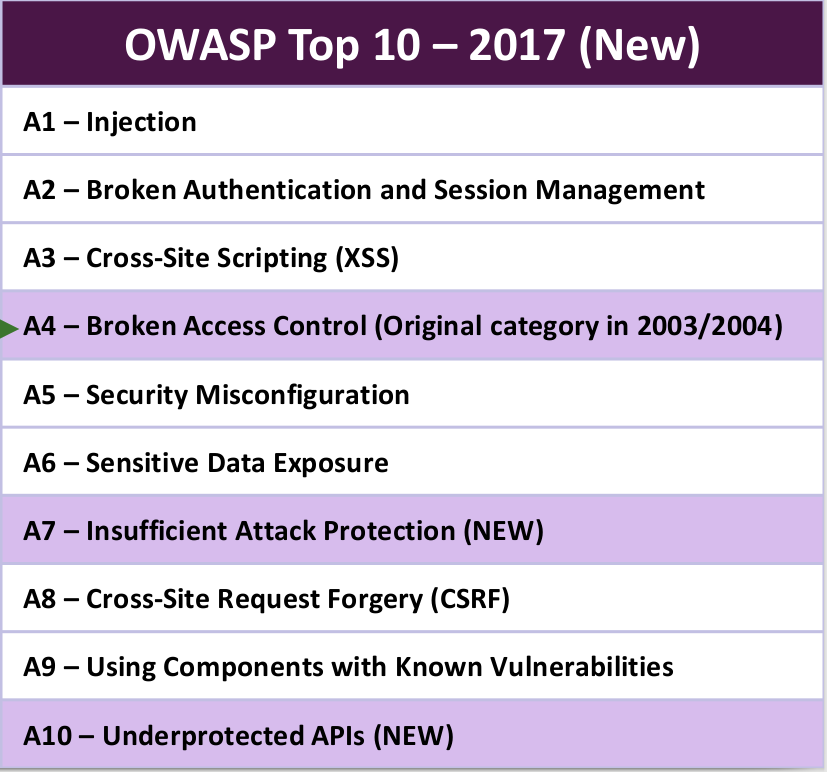
\includegraphics[scale=0.4]{images/10_menaces.png}
%  \caption{Chiffrement d'un flux avec une clé de taille $n = 11$}
%  \label{chiffrement}
%\end{center}
%\end{figure}







